\chapter{Overview and development of the Diplomatiq application}
\label{chapter:diplomatiq}

This chapter demonstrates the Diplomatiq social network application\footnote{The application is available on \emph{https://app.diplomatiq.org.}}, its specification, client-server architecture, features and development methods, and implementation details.

\section{Introduction}

\subsection{Personal goals and outline of this chapter}

I want Diplomatiq to be a long-term project. After finishing the university, I want to establish and lead a company responsible for the operation and further development of the social network, extending it with features supporting real-world diplomacy as well. I want to make changes for the better, providing a suitable platform for diplomacy, one of the main driving forces of our globalized world. In this chapter I outline Diplomatiq's vision to the future, as well as its target audience, specification, implemented features so far, and development details.

\subsection{Vision}

With the continuous advancement of today's computing power and data processing capabilities, and mass data sources like social networks, we become capable to detect new, important connections between seemingly unrelated actions and events of the world. Several studies has shown such event detection approaches regarding various topics, such as smart societies~\cite{smartsoc}, critical public infrastructure~\cite{tien2016detection}, and security threats in computer systems~\cite{merza2015investigative}. Analyzing data in a given domains even opens the possibility of predicting domain-specific events~\cite{6894591}.

Diplomatiq's long-term vision is to become an embedded, integrated system in diplomacy, providing tools for diplomats, and capable of detecting events of international relations on the global scale, based on its own data. In order to get there, it starts off as a domain-specific social network initially for prospective diplomats of the younger generation, Model United Nations participants. Then it gradually expands to real-world diplomacy as more and more career diplomats are invited into the application through MUN conferences. This creates the social base of its ecosystem. New features driving diplomatic adoption can be added progressively, further expanding the network. Once it is used by enough people in the simulated and the real diplomatic domains, the system will already hold data of great value. Analyzing this data, along with processing data added into the system in real time, would open possibilities to detect and predict global events.

\subsection{Target audience}

Diplomatiq's initial target audience is the participants of Model United Nations conferences. As previously assumed, the number of students who participate in and/or organize MUN conferences is probably in the order of millions, worldwide. However, supporting MUN conferences is also an entry step into real diplomacy. This means that in the future, Diplomatiq's target audience will expand to career diplomats, government officials, and diplomatic administrators as well.

\section{Long-term feature goals against competitors}

\subsection{Introduction}

As previously detailed, Diplomatiq has a direct competitor regarding MUN conference organization: the MyMUN application provides several kinds of features for MUN conference organizers and participants, and has an already established social base with its more than 100,000 members~\cite{mymunwebsite}. Although the long-term vision of Diplomatiq is much broader than the current scope provided by MyMUN, in the short run, Diplomatiq should be able to cope with MyMUN.

This section introduces planned features for a similar, but better social experience, than the one provided by MyMUN. Most of the features detailed below were not planned in detail, and were not implemented as part of the current version of Diplomatiq. However, I want to include them into this thesis to summarize the future scopes of Diplomatiq as well as the current ones. The actually implemented features of the framework is detailed in \Cref{section:specification}.

\subsection{Features for entities organizing conferences, associations, and clubs}

\subsubsection{Registering and administering MUN conferences}

In Diplomatiq, the basic organizational unit should be a \emph{conference}. Such conferences should be able to have multiple sessions, which is an actual manifestation of the conference as a few-day-long event. A conference should be able to have a flexible hierarchy of organizational roles in order to cope with the relatively high fluctuation of the organizational body of a conference due to students graduating and leaving the host institution.

\subsubsection{Grouping conferences into an MUN association}

An \emph{MUN association} is a group of conferences owned, organized and hosted by the same legal entity. The concept of an MUN association can mostly be applied when the same educational institution organizes multiple conferences: in this case, the institution can be regarded as an MUN association. The system should be able to handle all organizational aspects of creating and maintaining an MUN association, along with the necessary administration of its leadership and ownership. Similarly to conferences, the system should provide a flexible approach for handling organizational hierarchies.

\subsubsection{Hosting MUN clubs}

MUN clubs are extracurricular activities usually taking place weekly or more often, hosted by an MUN association (educational institution) usually within its own premises, for its own membes (studends). An MUN club provides an opportunity for junior MUN participants to develop their debating and other skills in order not to take part in a conference completely unprepared. Diplomatiq should be able to handle the administration and documentation of MUN clubs, encourage association members to take part as often as they can, and record students' MUN club performance in order to combine them into their conference recommendations.

\subsubsection{Administering the organization of a conference session}

Diplomatiq should cover all administrational requirements of organizing an MUN conference. This includes customizable participant application with assignable roles, and handling all financial aspects of the application procedure. Organizers should be able to set the participants' fee regarding their roles, with additional discounts. Fully custom payment classes should also be added for covering additional financial needs. The system should provide a way to refund participant fees in case of cancellations. It should also support creating flexible and complete financial reports covering the requirements of accounting. Regarding finances, the software should offer ultimate transparency, and should record every transaction to be audited later.

Delegates and chairs should be able to choose their country and committee preferences up to an allowed number configured by organizers. The system should provide an automated way of creating preliminary assignments of county-committee pairs and participants — based on organizational priority metrics and applicant preferences — even before a delegation is accepted or rejected, and allow the organizers to incorporate these assignment previews into their decisions regarding the delegation's or the delegate's acceptance to the conference. The final assignments should also be automatically created, with optional organizational modifications.

\subsubsection{Cross-selling additional services}

Diplomatiq should establish business relationships with local businesses, such as hotels, restaurants, and entertainment providers in order to provide delegates additional offers or entertainment packages for conferences, with optional discounts. The system should also be able to handle contractual relationships between such local businesses and the entity organizing the conference, and incorporate this into its financial system when calculating the comsummative participation fee for applicants. In essence, Diplomatiq should allow the cross-sales of its own business partners' services, and also the services of conferences' business partners. These services can later include travel insurance, flight tickets, and car rentals, similarly to MyMUN. In the long run, Diplomatiq should provide a concierge-like service for applicant delegations, with personalized travel, flight, and entertainment offers, taking over all paperwork from applicants, so they can concentrate on preparing to the conference.

\subsubsection{Conference awards}

It is common to award best delegates and best chairpersons of a committee or of the whole conference. For delegates, conference awards can be an important milestone for further conferences or even in their professional lives, therefore Diplomatiq should be able to store these awards. Also, the system should be able to officially certify that a delegate received such awards on a conference.

\subsubsection{Personalized conference items}

All MUN conferences involve personalized items, such as badges and placards. After the application and assignment procedure finished, the system should be able to produce all such personalized items as one, singular, printable artefact, sorted by the organizers' needs, in order to free organizers from manual batch work.

\subsubsection{Ordering conference items from Diplomatiq}

Diplomatiq should be able to carry out the printing, packaging and shipping operations of several types of conference items on demand. This includes badges and placards in printed, optionally laminated form, as well as pass holders, and conference awards. This way, conference organizers can outsource all — virtual and paper-based — administrative paperwork to Diplomatiq.

\subsubsection{Marketing operations}

The system should provide a sophisticated marketing toolset for conference organizers for advertising their conference, with optionally targeting participants based on their previous MUN history. It should offer multiple types of promotions, with multiple pricing tiers.

\subsubsection{Logging and auditing}

All actions recorded on Diplomatiq should be retriavable in a non-deniable, auditable manner. The platform should offer sophisticated search features for fetching the history of applicants, or organizational actions of a conference. Nevertheless, the principle of least privilege and access should be applied in every case: organizers should only access data they need to conduct their work, within only their conference.

\subsubsection{Providing catering, supplies, and infrastructure services for conferences}

In the long run, Diplomatiq should provide on-site services to conferences. These services can include catering services for lunch and for soirées, providing supplies for conferences such as mineral water and snacks, and even infrastructure services. Usually educational institutions do not even have wireless internet, let alone microphones, computers, and printers for every committee.

\subsubsection{Recording entire MUN conference sessions, producing commercials}

Diplomatiq should provide a data recording service for conferences, as part of its on-site services. Conferences produce lots of data: committee proceedings, resolutions, video recordings of ceremonies… On demand, Diplomatiq should be able to send a team to the conference with the tools to record the entire conference including committee work with the contribution and speeches of every delegates in every committees, ceremonies, soirées. Ultimately the \textquote{recorded package} should contain video and sound recordings, the exact record of all proceedings in committees, and all related paperwork, and serve as the record of the entire conference session. This recorded package then can be uploaded to Diplomatiq, and retrieved later for additional work on demand. The video and sound recordings of the conference can also be used to produce commercials, if the organizers order any such services, for later advertisement.

\subsection{Features for entities participating in conferences}

\subsubsection{Recommending conferences to delegates and chairpersons}

Diplomatiq should recommend conferences to delegates and chairpersons, based on their experience, and preferences they set in their profile settings. Recommendations can include sponsored and paid recommendations, as well as additional advertising of conferences. The platform should measure the efficiency of its organic and sponsored recommendations, and improve its targeting algorithms upon them.

\subsubsection{Public participant profile}

Participants often benefit from having an extensive MUN experience. Diplomatiq should provide audited profiles for delegates certifying their conference participations and and listing their awards, allowing conference organizers to see a CV-like summary of applicant delegates. Profiles should also contain organizational experience, if there is any.

\subsubsection{Membership programs and discounts}

Diplomatiq should provide a discount system for top delegates, delegations and conferences. Discounts can be participant fee discounts, or discounts for attached services, either way encouraging entities to strive for better performance.

\subsection{Features for non-MUN entities}

Similarly to Twitter and LinkedIn, Diplomatiq could also offer data licensing model for external parties interested in globally available, audited and verified data on Model United Nations. Later, simultaneously with the framework's expansion to real-world diplomacy, as the volume of data to be licensed also grows, more kinds of interested parties can be involved. In this model, Diplomatiq should offer anonymized data only.

\section{Specification and implemented features}
\label{section:specification}

\subsection{Introduction}

This section lists Diplomatiq's implemented features extensively, and can be regarded as a specification on how the system available on \emph{https://app.diplomatiq.org} should behave under different conditions. The section presents the features along the user journey of a user who registers the application, applies to a conference, then decides to organize a conference as well. Supplementary user flows, such as a user forgetting a password, are presented separately. At this point, I would like to point out that the goal of this thesis was to implement the framework on strong infrastructural and architectural foundations, but with \emph{a primitive, minimal feature set}.

\subsection{Registration}

The user visiting Diplomatiq arrives to a login screen, where they either logs in with their existing credentials or decides to register a new account. Diplomatiq offers registration and authentication based on email address and password only.\footnote{This was a technological decision justified by my security requirements. I will detail this decision's background in \Cref{chapter:security}.}

For registering a new account, the user needs to enter their valid, existing email address, their first and last name, and their password. After initiating the signup, they receive a success message about receiving an email with a link containing a long and secure email verification code. The user needs to click on that link and thus verify their email address before logging in to Diplomatiq, otherwise the system will not let them in.

If there is already a registered in Diplomatiq with the email address provided at registration, the application is obviously not able to register another user with that same email address. However in this case, the user is still notified that the registration was successful, and a verification email was sent to the provided email address — even though the email of course will not arrive. This is one of the many security measures to prevent malicious parties from obtaining the email addresses of registered users. Diplomatiq does not leak user emails in any way.

\subsection{First and second factor of authentication}

After the user verified themselves, they arrive to the login page of the application with their email address prefilled.\footnote{The lack of automatic login in this case is intentional. On the one hand, password-based cryptographic operations involved by the login process cannot be substituted with a simple link. On the other hand, I have put serious effort into implementing a zero-knowledge authentication protocol which makes it cryptographically impossible that the server impersonates the client. Sending a link to the user which provides them a fully authenticated session would contradict this.} After the user entered their password and clicked on \emph{Log in}, they receive an email with a two-factor authentication code.\footnote{In the future, I will incorporate a dedicated multi-factor authentication service, possibly Authy (https://authy.com).} After the user provided the valid authentication code, they are logged in to Diplomatiq, and is taken to the Dashboard.

\subsection{The Dashboard}

The Dashboard provides a summary about conferences the user takes part in or organizes. The two kinds of conferences are shown in two separate tab. In participant role, the user can see data about the conference (name, codename, dates, and venue address) and their committee seat (represented country in a committee) they applied to. The user can cancel their application in this view. If the user has not applied to any conferences, they are encouraged to apply to one in the empty state view of the participated conferences' list.

In organizer role, the user's organized conferences are listed with a name, codename, dates and venue address. Also, the number of applied participants is shown in a progress bar view, in the ratio of all announced committee seats of the conference. The organizer user can see the country matrix, which is a list of users occupying committee seats they applied to. The user can also cancel the conference from this view. If the user has not organized any conferences, they are encouraged to organize one in the empty state view of the organized conferences' list.

In the Dashboard's both views' right side, the user is encouraged to apply to a conference, or to organize one. This panel is always visible, regardless of the user current conferences, either in participant or in organizer role.

\subsection{The navigation bar}

The top navigation bar of the application hosts two elements. The application's logo is always visible, and if the user is logged in, navigates to the Dashboard, else it navigates to the login screen. If the user is logged in, the navigation bar dispalys a user menu as well. The user menu is a drop-down menu displaying the user's email address and having 4 navigation action buttons: \emph{Dashboard} (navigates to the Dashboard), \emph{Explore} (navigates to the view where users can apply to conferences), \emph{Settings} (navigates to the user settings), and \emph{Log out} (logs out the user and navigates to the login page).

\subsection{Applying to a conference}

Users can apply to announced conferences on the Explore page, which can be reached either via the user or from the Dashboard. On the Explore page, the conferences which the user can apply to are presented as a list, with their name and codename, dates, and venue address. Such conferences are conferences which are in the future, and the user has not applied to them yet. With the only button in a conference's row, a user can initiate the application process. This opens a modal showing the vacant committee seats of the conference, which the user can directly select and apply to, or abort the application process by closing the modal. After clicking on a seat's \emph{Apply} button, the application process is complete. The conference organizers are notified of the application via email.

\subsection{Organizing a conference}

Users can initiate organizing a conference from the Dashboard. On the opening modal, users should provide conference data, such as the conference's name and codename, its starting date and ending date, the address of the conference venue, and committees with seats. The dates can be provided as string in \emph{YYYY-MM-DD} form, or by an associated date chooser element. Dates are validated, so the start date can only be one day after the current date, and the ending date must not precede the starting date.\footnote{As there are one-day conferences, the end date can be the same as the start date.} For the venue address, users should provide the country, city, the address itself, and a postal code. The country is implemented as a search-assisted drop-down from a fixed set of countries according to the ISO 3166 standard.

Committees and their seats can be added on a per-committee basis, on a separate modal, providing the committee name and its codename. Adding a country creates a new form element, where the country's name can be provided. Once all countries in a committee are provided, the committee can be saved, and another committee can be added. After all committees are added, the conference can be saved, which also immediately opens the application to the conference.

\subsection{Cancelling a conference application}

The user can cancel their application to a conference on the Dashboard, on the participant role tab. Cancelling a conference application requires password-level authentication for assuring the identity and intention of the user: they need to provide their password to be able to cancel their application. This action sends an email to the conference organizer about the cancellation.

\subsection{Cancelling a conference}

The user can cancel one of their organized conferences on the Dashboard, on the organizer role tab. Cancelling a whole conference needs two-factor-level authentication for assuring the identity and intention of the user: they need to provide their password and enter the two-factor authentication code they received in email, in order to be able to cancel a whole conference. This action sends an email to all conference applicants about the cancellation.

\subsection{Password change}

Users can change their password on the Settings page, which can be reached from the user menu. Changing password needs password-level authentication: the user needs to provide their current password in order to be able to change it.

\subsection{Account deletion}

In case a user does not want to use Diplomatiq any more, they can delete their account, if they have no such conferences either as organizer or as participant, which ends in the future. Account deletion can be initiated on the Settings page, and requires two-factor-level authentication: they need to provide their password and enter the two-factor authentication code they received in email in order to delete their account.

\subsection{Password reset}

If a user forgot their password, they can reset it with an email-based password-reset flow, initiated from a modal on the login page. When the user provides their email address in the modal, and submits the form, they receive an email with a long and secure password reset link. Opening the link takes them to the reset password view, where they can supply a new password. After resetting a password, they are able to log in with the new password.

\section{Development and implementation details of the back end}

\subsection{Introduction}

Having already used Spring Boot in hobby projects, I had an explicit concept on how I want to build and layer the back end epplication. This section introduces the steps of setting up the Diplomatiq back end application — exposing an API over HTTPS, communicating with a database — from scratch until a publicly available application on the internet. Throughout the development, I strived to keep the quality, configurability and reliability of the application as high as possible. Security-related features and implementation details — such as authentication, authorization, additional security features for communicating over a HTTPS API, encrypted database entries, and additional web application security elements — of the application will be detailed in \Cref{chapter:security}.

\subsection{Setting up an empty Spring Boot application}

Since Spring Boot heavily advertises that since it needs minimal configuration due to its opinionated view of the platform and third-party libraries, it makes easy to start off with the framework. I wanted to make use of this, therefore I initialized an empty Spring Boot project with the help of Spring Initializr, which bootstraps projects with needing minimal configuration.\footnote{https://start.spring.io} I set up a Java-based project with Maven, using the latest released version of the framework. The project's group name has been \emph{org.diplomatiq}, its artifact name has been \emph{diplomatiq-backend}, and thus its full package name has been \emph{org.diplomatiq.diplomatiq-backend}. I chose JAR-packaging due to reasons detailed later, and set the required Java SDK version to Java 11.

\subsection{API concepts}

\subsubsection{Introduction}

Since Diplomatiq's API is primarily for internal use\footnote{In the future, Diplomatiq will provide a public API as well, but on different design principles.}, I was able to make design decisions without worrying about adoption aspects. Since Diplomatiq's own client is the only one who consumes this API, I was able to build non-conventional architectural and security solutions\footnote{The implemented security measures will be detailed in \Cref{chapter:security}.} into the API without concern for its usability for external developers. Nevertheless, this approach ultimately lead to an API with transparent, well-documented, easy-to-follow conventions, fitting well into Diplomatiq's security framework.

\subsubsection{Flat, RPC-like construction}

REST\footnote{Representational State Transfer} APIs work well those kinds of semantics when the server exposes \emph{resources} over an API, and clients use those resources in certain ways. However, this semantics carries several inconvenient abstractions of and assumptions about the data model and the operation of the underlying application, which can make the API inflexible. During the development of Diplomatiq's back end API, I intentionally avoided the REST semantics in favor of a flat, RPC-like\footnote{Remote Procedure Call} interface, exposing \emph{methods} instead of \emph{resources}. Every method is exposed via its own HTTP endpoint with a one-depth fixed path, relative to the base URI of the API, e.g. \emph{https://api.diplomatiq.org/password-authentication-init-v1}.

\subsubsection{JSON or binary communication}

I decided to use JSON as the primary format of communication between the client and the server due to its transparency and ubiquitous support. However, if the content sent or received is represented in a purely binary format — e.g. an image file or a cryptographic key —, it can be easier to send it in its binary format rather than serializing then deserializing, therefore these resources can be transferred as binary.

In Diplomatiq's API, I do not use content negotiation between the client and the server.\footnote{Content negotiation allows the server to expose data in different representations on the same URI, by the demands of the client.} Every exposed endpoint has a fixed semantics for receiving and sending data.

\subsubsection{GET, POST, and PUT methods only}

According to well-defined semantics below, I decided that the API endpoints should be callable either with the \emph{GET}, the \emph{POST} or the \emph{PUT} HTTP method.

\begin{itemize}
\item \emph{GET} methods are allowed to have query parameters, but no request body.\footnote{A GET request can not have a request body anyway.} Semantically, they should be used for getting data, and must never modify data.
\item \emph{POST} methods are allowed to have a request body, but no query parameters. Semantically, they should be used for creating or modifying remote objects.
\item \emph{PUT} methods are allowed to have both a request body and query parameters. Semantically, they should be used for uploading large amounts of binary data, with attached metadata as query parameters.
\end{itemize}

\subsubsection{Endpoint-level versioning}

The versioning of the API is implemented on a per-endpoint basis, in order to provide maximum flexibility. Every exposed endpoint's path ends with the endpoint's actual version — such as \emph{/login-v1} and \emph{/login-v2} —, meaning they are essentially different endpoints, and can have completely different semantics and differing behaviour. Since the API is meticuluosly documented\footnote{API documentation will be detailed later.} — and also only used by Diplomatiq clients — this should not cause any problems, instead it allows to gradually modify the API instead of needing to publish a new vesion of the entire API with every breaking change.

With endpoint-level versioning, endpoint deprecation can also be easier. After a new version of an endpoint was published — without client change necessary —, a new client using the new endpoint can be released, then the old version of the endpoint can be unpublished from the API. This workflow allows to think of API changes as step-by-step modifications instead of a new version of the entire interface. This results in the lack of versioning the interface as a whole.

\subsection{Implementation details of the API}

I used Spring Boot's built-in capabilities to implement the API itself. Since the API methods do not carry any resource-like semantics, they have been compartmentalized into controllers along authentication schemes and levels\footnote{The concept of authentication schemes and authentication levels is detailed in \Cref{chapter:security}.}. This means every method requiring the same authentication scheme and authentication level is placed in the same controller.

Endpoints are automatically exposed by Spring Boot, according to the controller methods' annotations. These annotations define each endpoints' path (e.g. \emph{/login-v1}), HTTP request method (e.g. \emph{POST}), and its consumed and produced value (e.g. \emph{application/json}).

Every input and output parameter of every endpoint is implemented as a separate class, unless the parameter is a simple value. The request and response objects are named unequivocally, based on the endpoint's name and version, i.e. the request object of the \emph{/login-v1} endpoint is \emph{LoginV1Request}, and its response object is \emph{LoginV1Response}. Marshalling and unmarshalling\footnote{Marshalling (serialization) means transforming an object's memory representation to a serialization format. Unmarshalling (deserialization) means transforming serialized object into memory reprepsentation.} is automatically performed by the Jackson library\footnote{https://github.com/FasterXML/jackson}, which is automatically configured by Spring Boot.

\subsection{Documenting the API}

I introduced and configured the \emph{springdoc-openapi} library\footnote{https://springdoc.org} for the automated documentation of the API according to the 3\textsuperscript{rd} version of the OpenAPI Specification~\cite{openapi-spec}. For human processing, the documentation is publicly available.\footnote{https://api.diplomatiq.org/openapi-documentation/v3/ui}

The OpenAPI documentation also has a format processable by machines, meaning I was able to automatically generate a fully functioning API client for the front end project, based on the exposed API documentation for machines.\footnote{https://api.diplomatiq.org/openapi-documentation/v3/api}

\subsection{Domain data model}

The domain data model of the application consists of the following entities:

\begin{itemize}
\item \lstinline{AuthenticationSession}
\item \lstinline{AuthenticationSessionMultiFactorElevationRequest}
\item \lstinline{Committee}
\item \lstinline{CommitteeSeat}
\item \lstinline{Conference}
\item \lstinline{Session}
\item \lstinline{SessionMultiFactorElevationRequest}
\item \lstinline{UserAuthentication}
\item \lstinline{UserAuthenticationResetRequest}
\item \lstinline{UserDevice}
\item \lstinline{UserIdentity}
\item \lstinline{UserTemporarySRPData}
\end{itemize}

\Cref{fig:data-model} displays a summary about Diplomatiq's entire data model with the entities' labels, labeled entity connections, and the connections' cardinalities.

For mapping objects and object relations to graphs, Diplomatiq uses the Neo4j-OGM library, built into the Spring Data Neo4j (SDN) project. SDN provides a fully-fledged data access layer handling database sessions and transactions transparently. Classes annotated with the \lstinline{@NodeEntity} annotation are automatically regarded as domain entities, thus incorporated into SDN's scope, and can be handled via \emph{repositories} providing convenient, automatically configured CRUD\footnote{Create, Read, Update, Delete} methods. For more convenient entity modeling, I defined a hierarchy of abstract classes for entities. \lstinline{AbstractIdentifiableNodeEntity} generates 32-character-long random alphanumeric identifiers; \lstinline{AbstractCreationRecordedNodeEntity} and \lstinline{AbstractExpiringNodeEntity} handles storing creation and expiration uniformly.

\begin{sidewaysfigure}[!p]
    \centering
    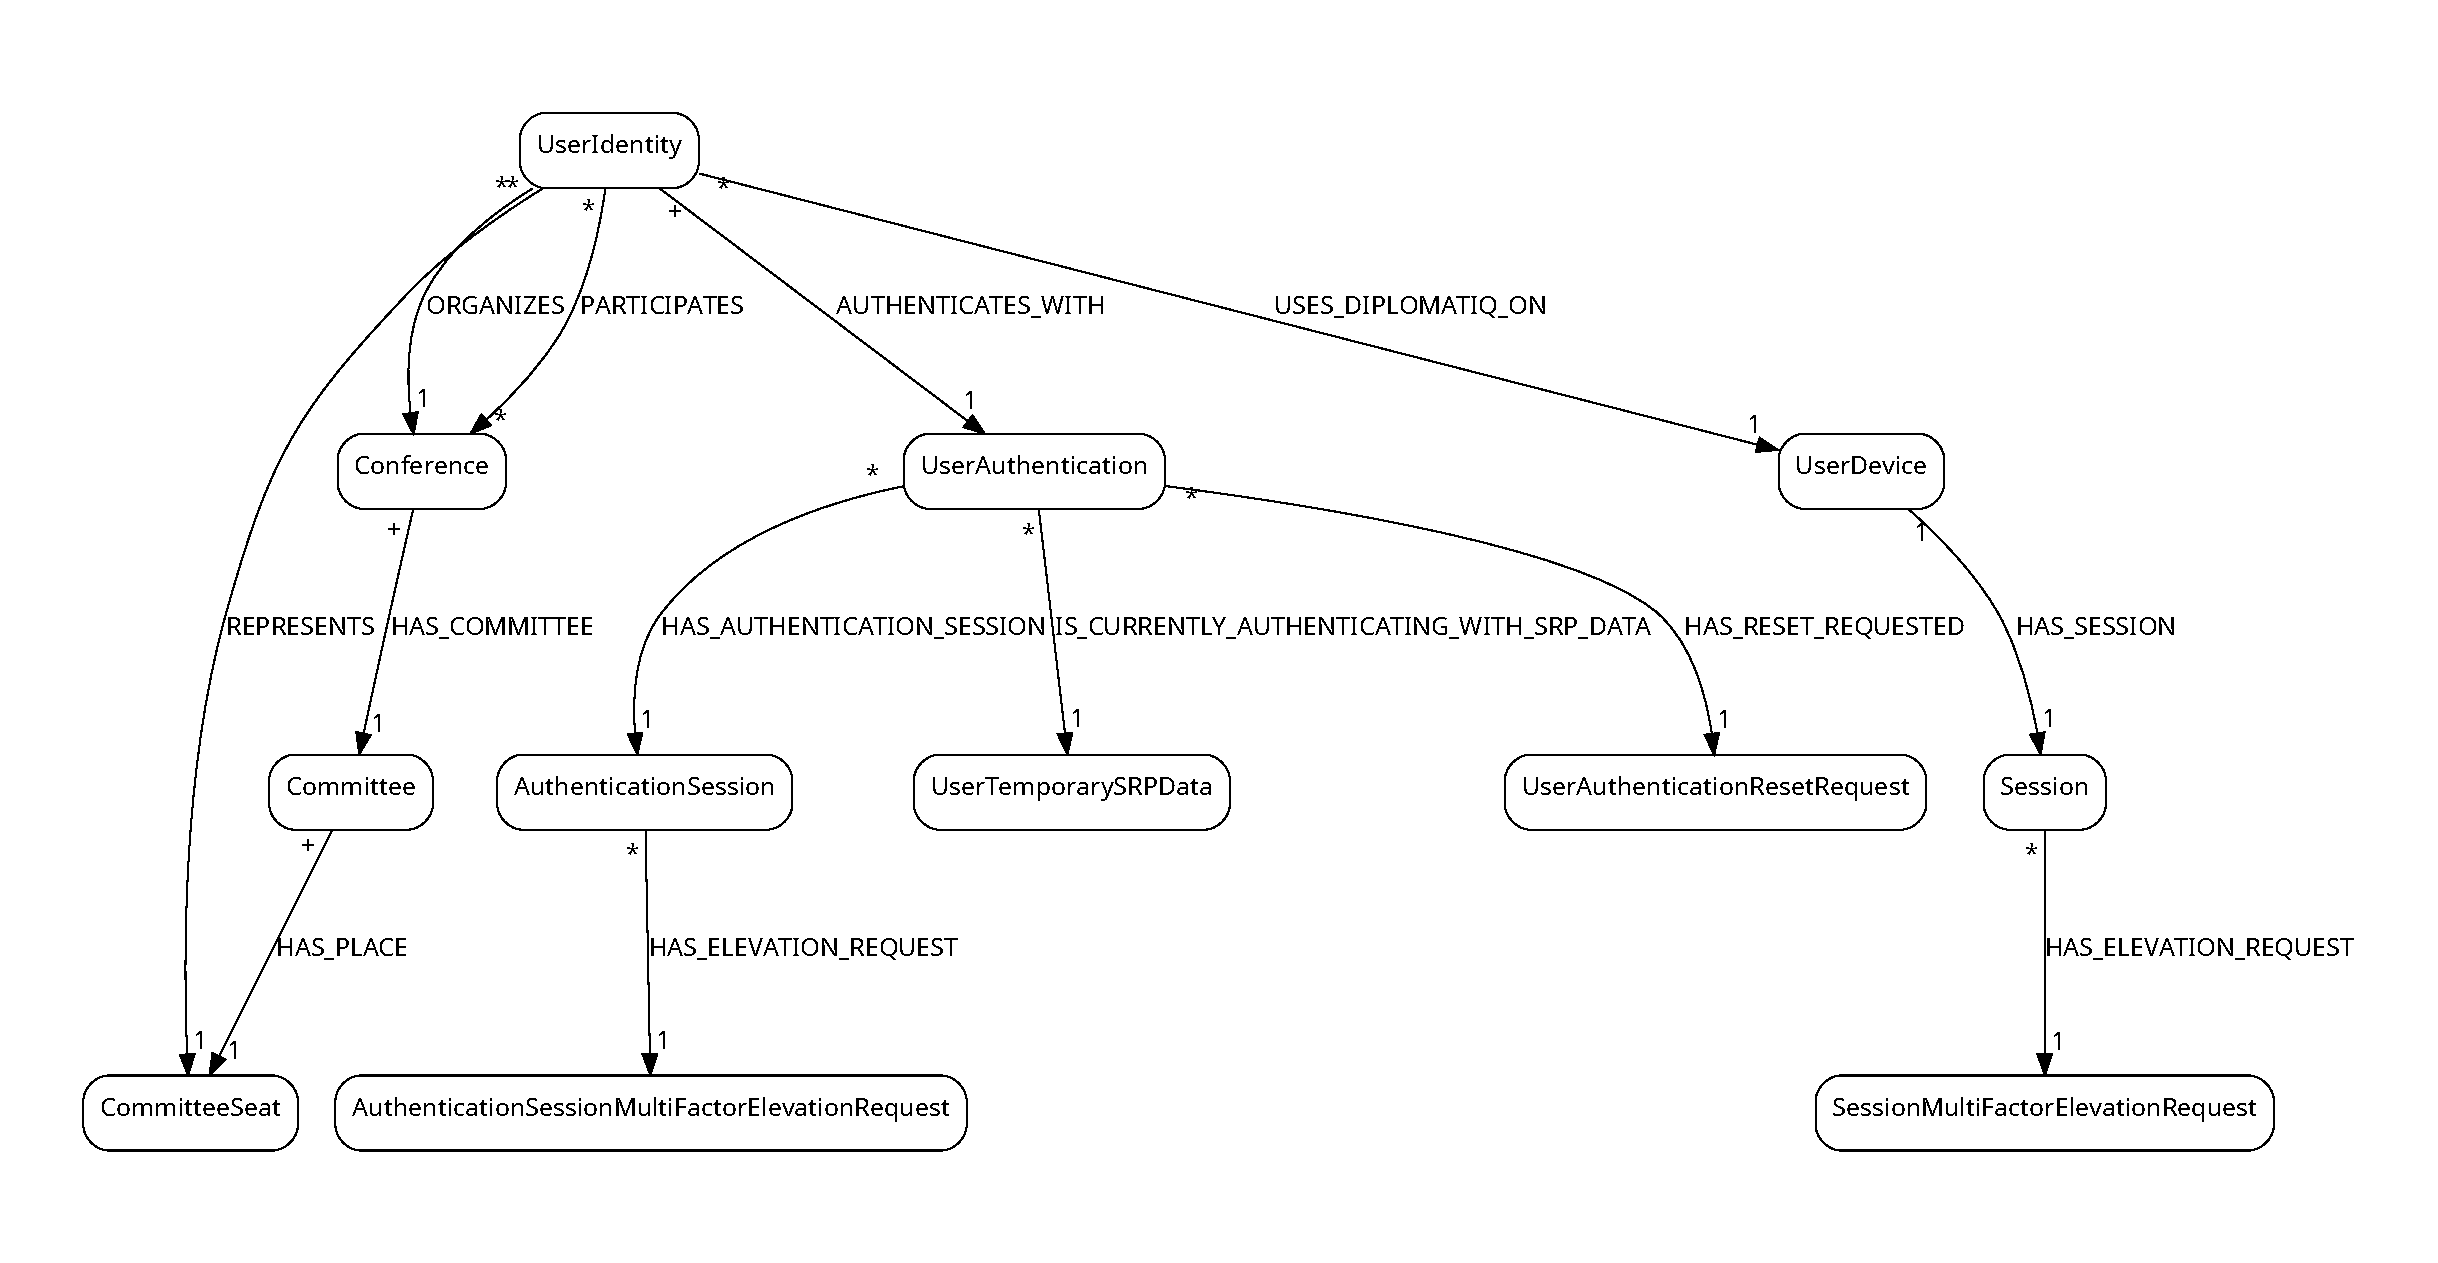
\includegraphics[width=\textheight]{figures/data-model.pdf}
    \caption{The data model of the Diplomatiq application}
    \label{fig:data-model}
\end{sidewaysfigure}

\subsection{Layering the application}

Maintaining a transparent implementation hierarchy is key to efficient software maintenance. Therefore I defined the following application structure from the API layer to the database layer\footnote{This structure excludes everything which are handled by the application server, or the Spring Boot framework or any related libraries, such as reading and writing HTTP requests and responses, and actually interacting with the database.}:

\begin{itemize}
\item \emph{Filters} forward or reject an incoming HTTP request, and play a key part in Diplomatiq's security architecture, which is detailed in \Cref{chapter:security}.
\item \emph{Controllers} handle HTTP requests and return HTTP responses. Thanks to the automated marshalling, the controller layer can be regarded responsible for converting JSON input to a POJO\footnote{Plain Old Java Object}, and forward it to the service layer (and vice versa).
\item \emph{Services} are the highest-level actors of the business logic layer (BLL). They act as transaction boundaries: if an exception is thrown within the service, the related database transaction is rolled back.
\item \emph{Engines} contain lower-level logic for performing specific computations.
\item \emph{Utilities} and \emph{helpers} represent the lowest levels of the BLL, and abstract frequently used functionalities, such as creating an entity in a uniform way.
\item \emph{Repositories} are lowest-level actors of the application hierarchy, representing the data access layer. They are responsible for reading from and writing to the database in a managed way.
\end{itemize}

\subsection{Error handling}

In the following, the term \emph{business error} denotes all errors that the client's and the server's joint business logic is built upon, essentially meaning all those errors which the client needs to be distinguish from each other. In Diplomatiq, errors which are lower level than business errors do not need to be exposed — and should not need to be exposed\footnote{Too detailed errors exposed by the API can reveal sensitive security properties of a system to an attacker.} — by the server, thus they are mapped to a suitable business error.

Business errors are handled in a semantically uniform way. One of my design principles was that the API either returns a success or an error, and I mapped this principle to the use two HTTP error codes only, where 200 means success, and 400 means error. In every case, the error response is an object consisting of a distinctive error code string, and optional retry information. Every business error has its own error code, thus the client can distinguish errors based on this error code. In case of an error which does not carry any specific semantics or its origin is unknown, the error code is \lstinline{InternalServerError}. Error codes are documented in the exposed API documentation.

\subsection{Configuration}

Most of the back end application's configuration has been externalized into configuration files or environment variables. Spring Boot supports externalized configuration well~\cite{spring-boot-reference-docs}. Database credentials and API keys are always stored in environment variables only, or they get a default, \textquote{dummy} value if their environment variables are not found. This makes development easier, since the local development environment can be set up with those dummy values, instead of needing to set up environment variables every time.

\subsection{Packaging and deployment}

Spring Boot provides two way of packaging an application: either as a traditional WAR\footnote{web application resource or web application archive} file, or a stand-alone, self-contained JAR\footnote{Java archive} file. The WAR file format is more suitable for deploying the software into a monolith application server hosting multiple web applications. The JAR file format is self-contained, meaning it encapsulates an embedded servlet container\footnote{The default servlet container for Spring Boot is Tomcat, but Jetty or Undertow are available as well~\cite{spring-boot-reference-docs}.}, and runs the actual Spring Boot application on this embedded application servlet container.

The back end application is packaged as a stand-alone JAR file, as this approach fits more into Diplomatiq's infrastructure: there is no need to deploy and maintain a fully-fledged Java application server. Instead, only a self-contained JAR file needs to be uploaded onto the web server, and the web server needs to be configured to start the application defined by the JAR, and forward all incoming requests to the application.

The deployment of the back end application is performed as part of the project's continuous delivery flow. Whenever the master branch of the repository is updated, the automated workflow defined in GitHub Actions eventually creates a distribution artefact. The final artefact is uploaded onto the \emph{staging} slot of the project's App Service in Microsoft Azure. Then the \emph{staging} slot's webserver instances are warmed up in order to receive production workload, meaning that the new version of the application is started on both instances. As soon as both instances reply to a continuous polling with a non-error response — meaning they are fully initialized —, the \emph{staging} slot is automatically swapped into production, resuting in no downtime during deployments.

\section{Development and implementation details of the front end}

\subsection{Introduction}

Having used the Angular framework throughout my career so far, I had a defined concept on how I want to build Diplomatiq's client application. Although the implemented application is relatively small and provides few features, I wanted to build the software on a high-quality foundation, so later it can be easily extended on demand.

\subsection{Creating an empty Angular application}

I bootstrapped an empty Angular application with Angular CLI.\footnote{https://cli.angular.io} The project has been named \emph{diplomatiq-frontend}. As part of the guided bootstrapping process, I added several modules to the application, such as routing, and set the project's stylesheet format to SCSS. Angular CLI created the folder structure of the project, and installed all necessary dependencies via NPM.

\subsection{Structuring the application}

\subsubsection{Components}

A routed Angular web application loads \emph{components} on configured paths: such components encapsulate a view displayed in the web browser and a logic of how the component works and reacts to user interactions~\cite{angular-reference-docs}. Components can be nested into each other, allowing developers to create complex application layouts. I tried to keep the component layer as thin as possible, in order to abstract all actual application logic into \emph{services}.

\subsubsection{Modules}

Angular applications are modular. \emph{Modules} are a set of components and configuration, which belong to one coherent application unit, a workflow, or closely related set of capabilities~\cite{angular-reference-docs}. Modularization can be beneficial in terms of compartmentalized application loading or application bundle size. However, the front end application of Diplomatiq consists of only one \emph{root} module, making no use of those advantages.

\subsubsection{Services}

Services are application classes containing logic. Besides components, most of Diplomatiq's front end application code is in services, which are responsible for data manipulation, and transitively — through a dedicated API service — for calling the back end API as well. Services are usually injected into components or other services with dependency injection.

\subsection{API access and error handling}

I implemented a dedicated service for performing API calls. This service exposes the endpoints of the back end's API, which is compartmentalized by authentication schemes and levels. As the API client is automatically generated using the \emph{openapi-generator}\footnote{https://github.com/OpenAPITools/openapi-generator} tool, this compartmentalization is visible in the client as well, meaning the API service actually exposes additional \textquote{services} instead of the endpoints themselves. The exposed services are the partial APIs compartments — each with endpoints with the same authentication scheme and level —, and they are the ones providing the actual endpoint stubs.

The \emph{openapi-generator} tool can be configured to generate code for several libraries and frameworks, including Angular. Although, the server stubs generated for Angular did not offer any way for attaching dynamically computed headers to the server request, as it did not provide any way to add before-request or after-request hooks to the generated code. This is a requirement for Diplomatiq, because the request's cryptographic signature — required by the back end API as a header — is not a static, configurable value, but needs to be computed from the request dynamically. Therefore I configured the generator to generate code utilizing the Fetch API~\cite{fetchapi}, a modern, native browser API for performing asynchronous, cancellable network requests.

API errors are handled in an after-request hook of the generated API client. If the API response has a different HTTP response code than 200, a JavaScript error is thrown with its error message set to be the received error code. If the received error response has no error code, or is not an error which conforms to the Diplomatiq error scheme mentioned earlier — meaning the back end application is incapable even to produce a business error for some reason —, the \lstinline{InternalServerError} error code is set.

\subsection{Packaging and deployment}

Angular provides sophisticated build tools, capable of generating all source files of the application into one bundle with \emph{webpack}\footnote{https://webpack.js.org}, one of today's most popular JavaScript bundler. Therefore, building the distribution artefact essentially means that only an Angular-specific command needs to be invoked, which builds the application bundle, and copies it with additional assets, such as images and icons, into a folder, usually called \emph{dist}. The contents of the \emph{dist} folder contains the entire application, and can be uploaded to a web server.

Similarly to the back end project, the deployment of the front end application is performed as part of the project’s continuous delivery flow. Whenever the master branch of the repository is updated, the automated workflow defined in GitHub Actions eventually creates a distribution artefact. The final artefact is uploaded onto the staging slot of the project’s App Service in Microsoft Azure. After the files were placed into the webserver's public folder, and ready to be served to users, the staging slot is automatically swapped into production, resulting in no downtime during deployments.\footnote{In case of static web applications, there is no need to warm up the instances, as there is no back end application to start on the web server. However, Azure copies static files into its webservers' public folder by taking the webserver offline, and I wanted to avoid the downtime caused by that.}
